\documentclass[11pt, a4paper]{article}
\usepackage{graphicx, fullpage, hyperref, listings}
\usepackage{appendix, pdfpages, color}

\usepackage{tocloft}            % This squashes the Table of Contents a bit
\setlength\cftbeforesecskip{3pt}

\definecolor{MyLightYellow}{cmyk}{0,0.,0.2,0}

\setlength{\parskip}{4pt}        % sets spacing between paragraphs
\interfootnotelinepenalty=500    % this prevents footnotes breaking across pages

\title{
\includegraphics[width=0.4\textwidth]{UnivCrest}
        \\Experiment 81 - Design of a Feedback Control System}          % <<<<<<<<< change the title as appropriate
\author{%\textcolor{red}{Student ID 200123456 (Group 999)}                % <<<<<<<<< your ID and group number
        \\  \textcolor{red}{ELEC273}\footnote{\textcolor{red}{IMPORTANT: In a standard technical report, you would need to include here your personal details as the author of the document. However, remember that marking of coursework is anonymous and therefore you should remove this part before submitting your report for Year 2 labs! Do not include your name, student ID, email address or any other personal information.}}}                                    % <<<<<<<<< module code
\date{\tiny{\today}}

\begin{document}
\begin{titlepage}
\maketitle
\addtocontents{toc}{\protect\thispagestyle{empty}} % because we don't want a page number on the title page
                                                   % Thanks to Huang Shanyue for suggesting this

\begin{abstract}
In this report, P model, PI model and PID model was utilized to design controllers in Matlab SimuLink. A high order plant was set to be simulated to find its unit-step response directly. FOPDT method was used to approximate the original response and to find the suitable parameters. It was investigated that comparing with P model, PI model seems to have higher OS\% but with nearly removed steady error. PI model shows more expected ability to against disturbance because of less Max value, nearly zero steady error compared with P model. Finally, a PID model was designed to make the anti-disturbance ability of the system to be as high as possible.
\end{abstract}

\fbox{
\begin{minipage}{0.9\linewidth} \footnotesize
\begin{center} \textbf{Declaration} \end{center}
I confirm that I have read and understood the University's definitions of plagiarism and collusion from the Code of Practice on Assessment. I confirm that I have neither committed plagiarism in the completion of this work nor have I colluded with ant other party in the preparation and production of this work. The work presented here is my own and in my own words except where I have clearly indicated and acknowledged that I have quoted or used figures from published or unpublished sources (including the web). I understand the consequences of engaging in plagiarism and collusion as described in the Code of Practice on Assessment (Appendix L).
\end{minipage}
}

\thispagestyle{empty}
\newpage
\tableofcontents
\end{titlepage}


%-------------------------------------------------------------------------------------------------------
\section{Introduction}
%-------------------------------------------------------------------------------------------------------


In this lab, control systems with a proportional and proportional-integral control was designed and simulated with MATLAB Simulink.\cite{ref:lab} 

\subsection{Background}

Control systems are everywhere and generally used to achieve control behavior to make the system acting as it is supposed to do. In general, there are two types of systems. One is open-loop systems which do not have a feedback from the result. They act with the logic set but can not fix errors automatically. This may mean that, if the errors of the system can be accumulated while the system continuing. Therefore, this kind of system is not suitable for some persistent running cases. The other type is close-loop systems, which have the output of their result as one of their input. This feedback mechanism makes them can automatically adjust themselves with a typical error of the output.

\begin{figure}[htbp]     \begin{centering}
    \includegraphics[width=0.5\textwidth]{1.png}
    \caption{\label{Fig:control}Control Model \cite{ref:lab}}
    \end{centering}
\end{figure}

Figure \ref{Fig:control} displays the general structure of a close-loop control model. In this model, the output is sent back to the input before the controller. After that, there could be an actuator and some disturbance being input into the system. Then, the plant which indicates the object of machine that needed to be controlled. The output of the result will be collected by sensors with possible errors.

This kind of control behavior is widely used in industry for achieving the control process with feedback to provide a sustainable and reliable control service. Therefore, it is important to learn and practice the design of such close-loop control systems.


\subsection{Objective}

The objectives of this lab was, firstly, get a approximate model of a high order open-loop system using First-order Plus Time delay (FOPDT) model. After that, proportional (P) controller, proportional-integral (PI) controller and proportional-integral-derivative (PID) controller will be designed and evaluated.


\subsection{method}

\begin{equation}
G(s) = \frac{K}{(Ts+1)^2}
\label{eq:trans}
\end{equation}

According to the lab script \cite{ref:lab}, the plant can be described by a transfer function, which is shown as Equation \ref{eq:trans}. In this equation, K presents the day of birth while T indicate the month of birth, in this case it is 4 and 9 accordingly.

%-------------------------------------------------------------------------------------------------------
\section{Part 1}
%-------------------------------------------------------------------------------------------------------
\subsection{Open Loop Respond}

\subsubsection{Method and procedure}

\begin{figure}[htbp]     \begin{centering}
    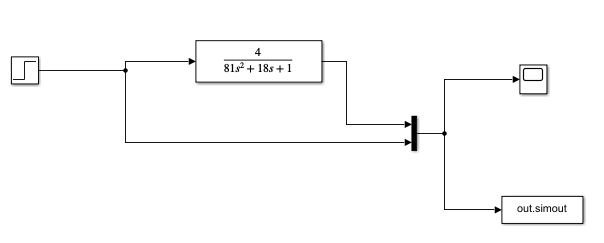
\includegraphics[width=0.5\textwidth]{p1_1.png}
    \caption{\label{Fig:p1_1}Open Loop Simulink model}
    \end{centering}
\end{figure}

Figure \ref{Fig:p1_1} shows the Simulink model of the direct simulation of open loop respond of the plant. As it shown in the picture, an unit-step change was generated and be input into the plant transfer function. After the plant, the signal was import into a scope to display the respond. Meanwhile, the data was also output to the workplace via a simout module.

\subsubsection{Result and Comment}

\begin{figure}[htbp]     \begin{centering}
    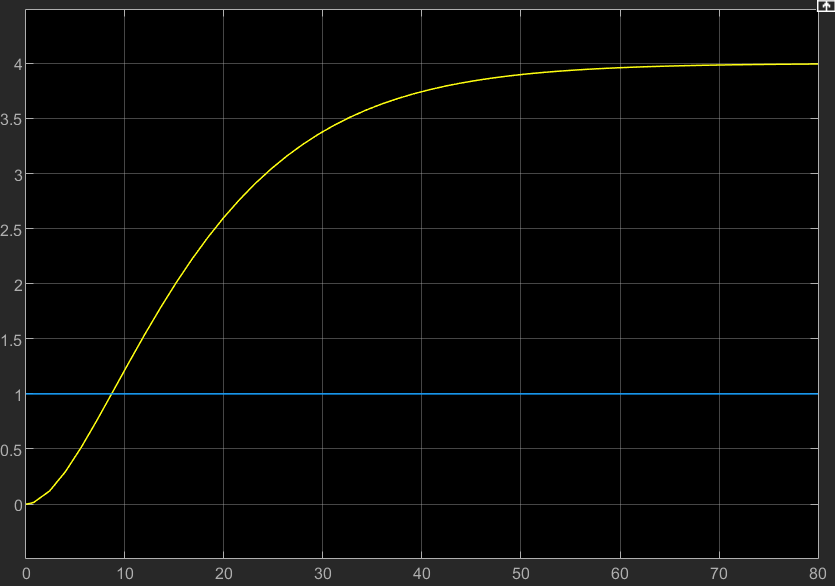
\includegraphics[width=0.5\textwidth]{p1_1_r.png}
    \caption{\label{Fig:p1_1_r}Result of Open Loop Simulink model}
    \end{centering}
\end{figure}

As it shown in the Figure \ref{Fig:p1_1_r}, the yellow line presents the respond of the transfer function while the blue line indicates the input unit step.

From Figure \ref{Fig:p1_1_r}, it can be indicated that when the input jumped from 0 to 1, the overall response begin to increase from 0. The increase of the respond with time firstly become quick and then become slow before approaching 4. Finally, after around time 70, the result was stable at 4. 

Theoretically, the expected result is a expression of the convolution of unit-step and plant. In transfer function, it should be the multiple of the transfer function of unit-step and the plant, as it shown in Equation \ref{eq:trans_1}.

\begin{equation}
Y(s) = \frac{K}{T^2s^3+2Ts^2+s}
\label{eq:trans_1}
\end{equation}

Equation \ref{eq:trans_1} can be classified into the following form with factorization.

\begin{equation}
Y(s) = \frac{K}{s}-\frac{K}{s+\frac{1}{T}}-\frac{\frac{K}{T}}{(s+\frac{1}{T})^2}
\label{eq:trans_2}
\end{equation}

In the time domain, Equation \ref{eq:trans_2} can be expressed as Equation \ref{eq:trans_3}.

\begin{equation}
y(t) = K-Ke^{-\frac{1}{T}t}-\frac{K}{T}e^{-\frac{1}{T}t}t
\label{eq:trans_3}
\end{equation}

From Equation \ref{eq:trans_3}, it can be inferred that this function is convergence at K. This result was similar to simulation because the convergence value is about 4 according to Figure \ref{Fig:p1_1_r}.

\subsection{FOPDT Approximation}

\subsubsection{Method and procedure}

From the Equation \ref{eq:trans_3}, the derivative and second order derivative can be calculated as Equation \ref{eq:trans_4} and Equation \ref{eq:trans_5}.

\begin{equation}
y'(t) = \frac{K}{T^2}e^{-\frac{1}{T}t}t
\label{eq:trans_4}
\end{equation}

\begin{equation}
y''(t) = \frac{K}{T^2}e^{-\frac{1}{T}t}(1-\frac{t}{T})
\label{eq:trans_5}
\end{equation}

From Equation \ref{eq:trans_5}, it can be found that the inflection point is achieved at time T, while the slope is k/Te, in this case, they are 9 and 0.1635. The tangent line pass by (t, 0.2642K), which is (9, 1.057) in this case.


\begin{figure}[htbp]     \begin{centering}
    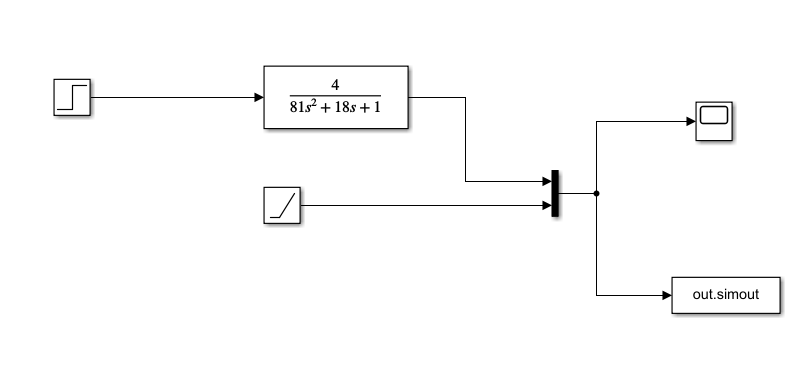
\includegraphics[width=0.5\textwidth]{p1_2.png}
    \caption{\label{Fig:p1_2}Tangent Line for Response}
    \end{centering}
    
\end{figure}

We use the simulation in Figure \ref{Fig:p1_2} to verify the computation of the tangent line. As it shown from the following picture \ref{Fig:p1_2_r}, the tangent line can suit the original respond. 

\begin{figure}[htbp]     \begin{centering}
    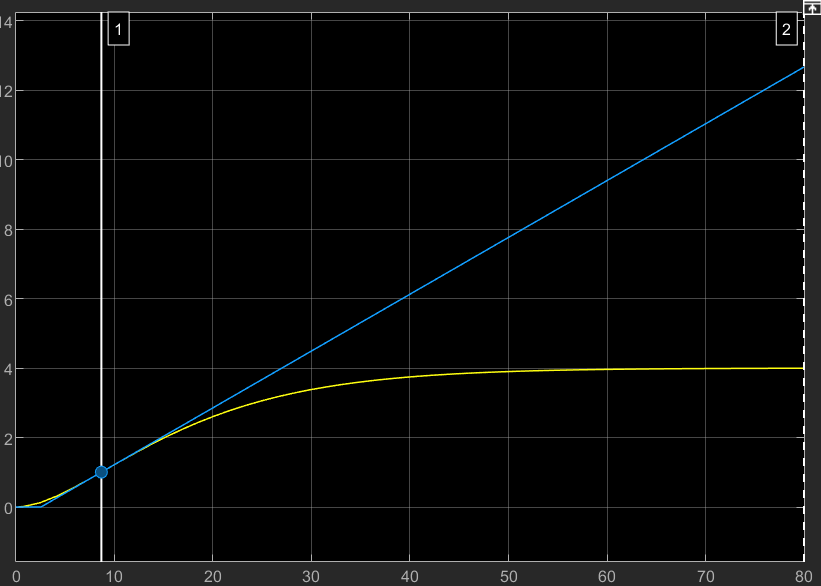
\includegraphics[width=0.5\textwidth]{p1_2_r.png}
    \caption{\label{Fig:p1_2_r}Tangent Line for Response Result}
    \end{centering}
    
\end{figure}

The parameters of FOPDT including the process delay time $t_{d}$, the process time $T_{p}$ and the process gain $K_{p}$ can be then calculated.


\begin{table}[htbp]
\caption{Parameters of FOPDT}
\label{tab:para_1}
\begin{center}
\begin{tabular}{ccc}
\hline
 $t_{d}$      & $T_{p}$       & $K_{p}$   \\
\hline
 2.535         & 24.465          &  4         \\

\hline
\end{tabular}
\end{center}
\end{table}

\begin{equation}
G(s) = \frac{K_{p}e^{-t_{d}S}}{T_{p}s+1}
\label{eq:FOPDT}
\end{equation}

With these parameters and Equation \ref{eq:FOPDT}, we built the FOPDT model to approximate the result. The build method was shown in the following Figure \ref{Fig:p1_3}.

\begin{figure}[htbp]     \begin{centering}
    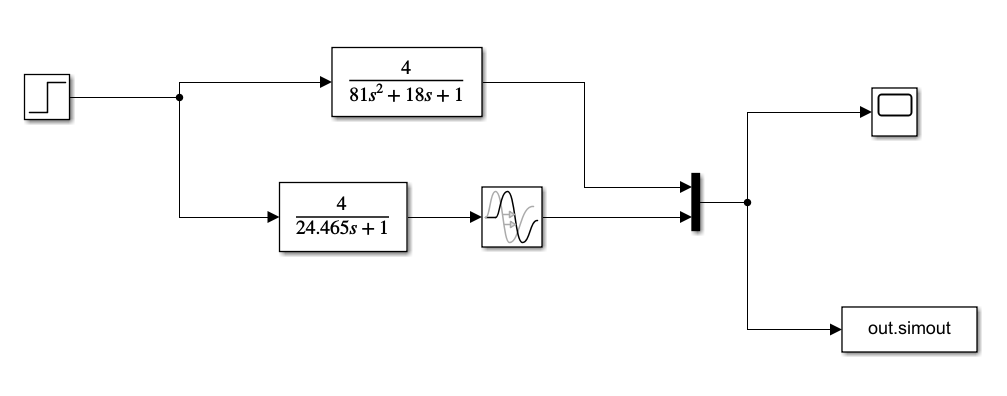
\includegraphics[width=0.5\textwidth]{p1_3.png}
    \caption{\label{Fig:p1_3}Simulink of FOPDT}
    \end{centering}
    
\end{figure}

As it shown in Figure \ref{Fig:p1_3}, a trans fcn module was firstly used to simulate the G(s) and then a delay module was used to simulate the delay part. After that, these two signal were sent to one scope to display.


\subsubsection{Result and Comment}

\begin{figure}[htbp]     \begin{centering}
    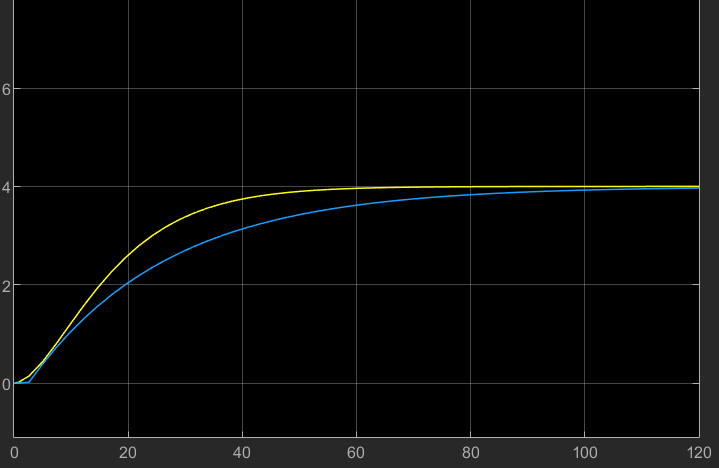
\includegraphics[width=0.5\textwidth]{p1_3_r.png}
    \caption{\label{Fig:p1_3_r}Simulink Result of FOPDT}
    \end{centering}
    
\end{figure}

Figure \ref{Fig:p1_3_r} shows the result of FOPDT model, while the yellow line shows the direct simulation of the plant and the blue line shows the FOPDT approximation. It can be indicated that these two result are nearly the same so that the FOPDT seems to be effective in simulate high order system.

From Figure \ref{Fig:p1_1_r} and Figure \ref{Fig:p1_3_r}, the steady-state error, \%OS, settling time $T_{s}$, and the rise time $T_{r}$ can be classified in to Table \ref{tab:resp_1}.

\begin{table}[htbp]
\caption{Parameters of FOPDT}
\label{tab:resp_1}
\begin{center}
\begin{tabular}{c||cccc}
\hline
 Model   &    OS\%      & $T_{r}$       & $T_{s}$   &  steady error \\
\hline
Open-loop  &   0         & 30.5          &  52.8     &  0     \\
FOPDT  &   0         & 53.5          &  98.5     &  0     \\
\hline
\end{tabular}
\end{center}
\end{table}

Table \ref{tab:resp_1} displays the comparison between the effect of Open-loop situation and FOPDT. It can be further indicated that the $T_{r}$ and $T_{s}$ of FOPDT are large than actual. But in generally, it is suitable for approximation.

\section{Part 2}

\subsection{Method and procedure}

To design a P controller, the most important thing to do is to settle the gain of the controller. According to FOPDT model, the recommended value of gain is determined by $\frac{T_{p}}{t_{d}}$. From the information of Table \ref{tab:para_1}, the value can be calculated to be 9.65. In this experiment, as we also need to compare the result of different controller parameters, two other P controllers were set with 7.65 and 11.65 to investigate the effect of changing this parameters of the P controller.

\begin{figure}[htbp]     \begin{centering}
    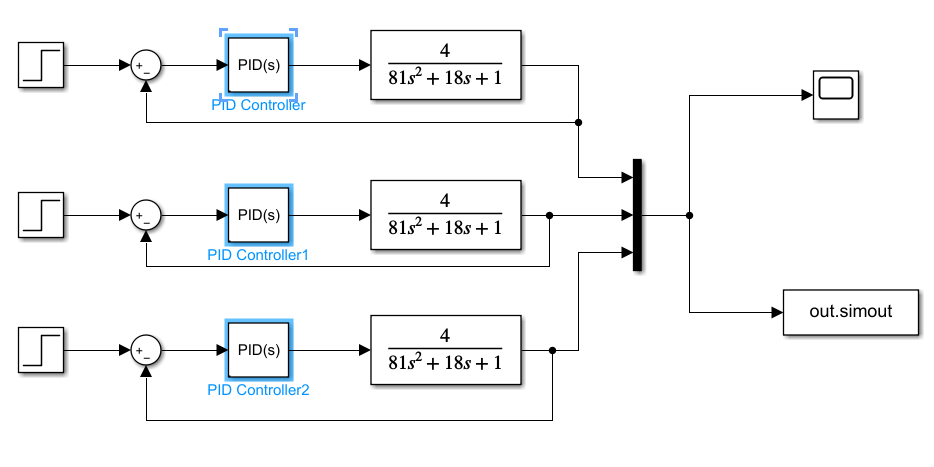
\includegraphics[width=0.5\textwidth]{p2.png}
    \caption{\label{Fig:p2}Simulink Model of P Controllers}
    \end{centering}
    
\end{figure}


\begin{table}[htbp]
\caption{Controller Gain}
\label{tab:pid}
\begin{center}
\begin{tabular}{ccc}
\hline
 PID Controller      & PID Controller 1       & PID Controller 2   \\
\hline
9.65         & 7.65         &  11.65         \\

\hline
\end{tabular}
\end{center}
\end{table}

Table \ref{tab:pid} displays the P value of these three controller, while Figure \ref{Fig:p2} shows the structure of how these three controllers being built. Similar to the above process, an unit-step and the result was import in to the P controller before the plant. The result was exports to scope to display.



\subsection{Result and Comment}

\begin{figure}[htbp]     \begin{centering}
    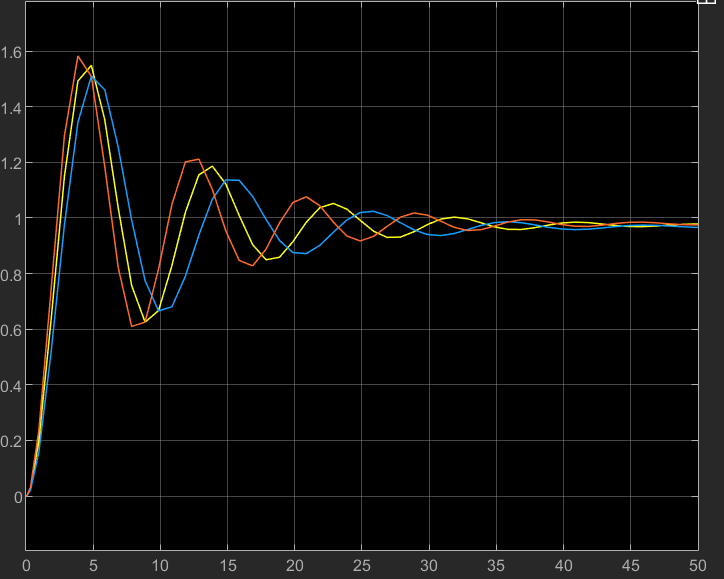
\includegraphics[width=0.5\textwidth]{p2_r.png}
    \caption{ \label{Fig:p2_r}Simulink Result of P Controllers}
    \end{centering}
   
\end{figure}

Figure \ref{Fig:p2_r} presents the result from the simuLink model in Figure \ref{Fig:p2}, while the yellow line represents the PID Controller, blue line represents the PID Controller 1, and the red line represents the PID Controller 2. It can be indicated from the figure that the red line acts quick than the other two lines and it achieve the stable condition much earlier than the other two lines. This may indicate that the larger the P gain, the more quick (strong) the controller can adjust the plant. Additionally, it can be noticed that the amplitude of the red line is greater than the other two cases. This may means that the larger the P value, the more shake would be generated before stable.

\begin{table}[htbp]
\caption{Parameters for different Kp}
\label{tab:resp_2}
\begin{center}
\begin{tabular}{c||cccc}
\hline
Gain   &    OS\%      & $T_{r}$       & $T_{s}$   &  steady error \\
\hline
7.65  &   50\%         & 2.0          &  25.7     &  0.032     \\
9.65  &   54\%         & 1.8          &  28.3     &  0.025     \\
11.65  &   58\%         & 1.6          &  28.7     &  0.021     \\
\hline
\end{tabular}
\end{center}
\end{table}

From Table \ref{tab:resp_2}, it can be shown that, with the increasing of P parameters, the OS\% and $T_{s}$ increases, while the $T_{r}$ and steady error decreases. The increase of OS\% indicates that the more gain, the more shaking amplitude. The decreasing $T_{r}$ indicates that the greater the gain, the quick the quicker the system can recover from effect. The increasing $T_{s}$ means that Greater gain can bring the system earlier to get into a stable condition. However, the decreasing steady error shows that the final state can be not equal to the ideal one.


\section{Part 3}

\subsection{Method and procedure}

From the FOPDT part, it can be conducted that one possible value for the gain $K_{p}$ and $K_{I}$ in PI case, while $K_{p}$ equals $0.9\frac{T_{p}}{t_{d}}$ and $K_{I}$ equals $0.27\frac{T_{p}}{t_{d}^2}$. Therefore, the value of $K_{p}$ and $K_{I}$ in our case can be calculated to be 8.69 and 1.03. 

\begin{figure}[htbp]     \begin{centering}
    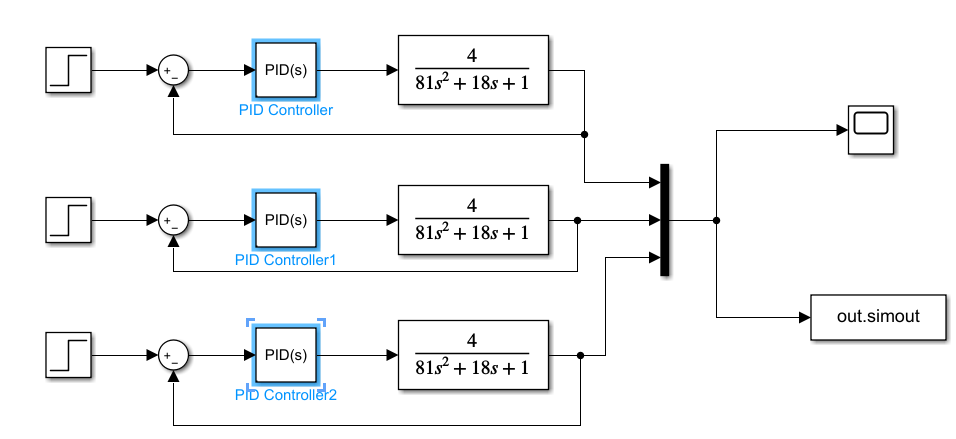
\includegraphics[width=0.5\textwidth]{p3.png}
    \caption{\label{Fig:p3}Simulink Model for PI controller}
    \end{centering}
    
\end{figure}



\begin{table}[htbp]
\caption{$K_{I}$ with $K_{p}$ equals 8.69}
\label{tab:3_1}
\begin{center}
\begin{tabular}{ccc}
\hline
 PID Controller      & PID Controller 1       & PID Controller 2   \\
\hline
0.53         & 1.03         &  1.53         \\

\hline
\end{tabular}
\end{center}
\end{table}


\begin{table}[htbp]
\caption{$K_{p}$ with $K_{I}$ equals 1.03}
\label{tab:3_2}
\begin{center}
\begin{tabular}{ccc}
\hline
 PID Controller      & PID Controller 1       & PID Controller 2   \\
\hline
7.69         & 8.69         &  9.69         \\

\hline
\end{tabular}
\end{center}
\end{table}

Figure \ref{Fig:p3} shows the method one simulink to simulate a PI controller. To investigate the properties of the PI controller, we firstly kept the value of $K_{p}$ at 8.69 and change the value of $K_{I}$ as shown in Table \ref{tab:3_1}. Then the value of $K_{p}$ was kept at 1.03 and the value of $K_{I}$ varied as shown in Table \ref{tab:3_2}.

\subsection{Result and Comment}

\subsubsection{Change K_{I}}

\begin{figure}[htbp]     \begin{centering}
    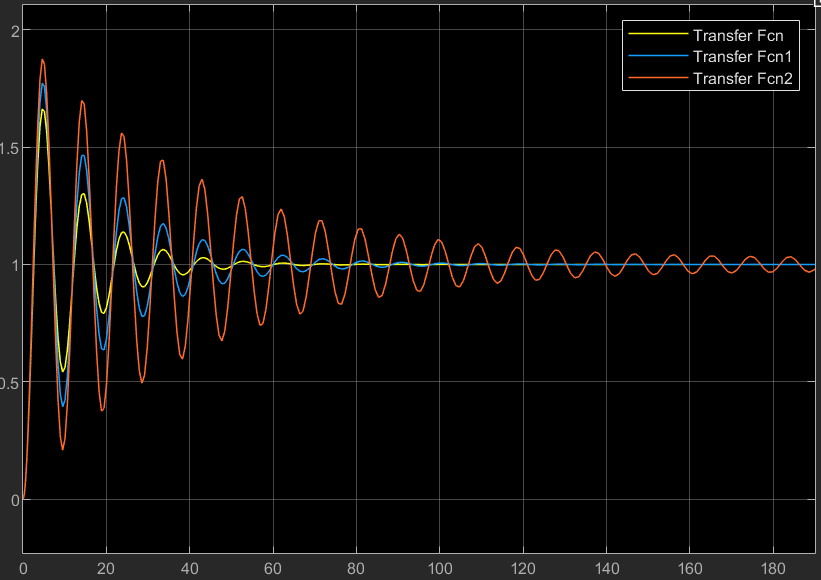
\includegraphics[width=0.5\textwidth]{3_1.png}
    \caption{ \label{Fig:p3_1}Result from $K_{p}$ equals 8.69}
    \end{centering}
   
\end{figure}

Figure \ref{Fig:p3_1} shows the result of keeping $K_{p}$ and changing $K_{I}$. It can be noticed that the larger the $K_{I}$, the stronger shaking would be. Besides, the system with a larger $K_{I}$ tends to take longer time to make the system back to the stable condition.


\begin{table}[htbp]
\caption{Result with different $K_{I}$}
\label{tab:resp_3_1}
\begin{center}
\begin{tabular}{c||cccc}
\hline
$K_{I}$   &    OS\%      & $T_{r}$       & $T_{s}$   &  steady error \\
\hline
0.53  &   65.83\%         & 1.6          &  68.61     &  0     \\
1.03  &   77.68\%         & 1.6          &  105.9     &  0     \\
1.53  &   95.01\%         & 1.6          &  $\infty$     &  0     \\
\hline
\end{tabular}
\end{center}
\end{table}


From Table \ref{tab:resp_3_1}, it can be found that with the increasing of $K_{I}$, the OS\% increases, the $T_{r}$ remains, $T_{s}$ increases and the steady errors are all zero. The increasing of OS\% indicated a stronger shake for the overall system. However, the steady error was effectively removed by adding the Integral part. The increasing of $T_{s}$ means that the adding $K_{I}$ can result in long time to recover to the stable state. If the value of $K_{I}$ is set for too large, this may result in a always shaking behavior.


\subsubsection{Change K_{p}}


\begin{figure}[htbp]     \begin{centering}
    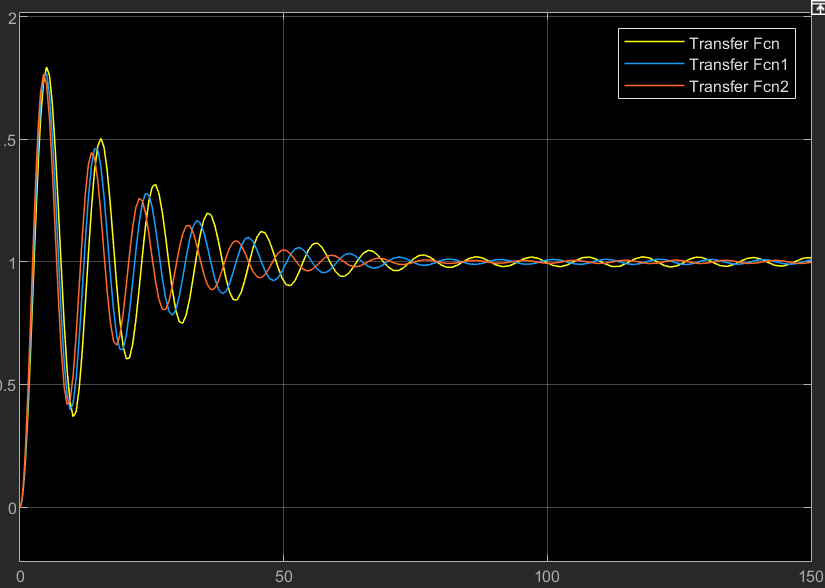
\includegraphics[width=0.5\textwidth]{3_2.png}
    \caption{\label{Fig:p3_2}Result from $K_{I}$ equals 1.03}
    \end{centering}
    
\end{figure}

\begin{table}[htbp]
\caption{Result with different $K_{p}$}
\label{tab:resp_3_2}
\begin{center}
\begin{tabular}{c||cccc}
\hline
$K_{p}$   &    OS\%      & $T_{r}$       & $T_{s}$   &  steady error \\
\hline
7.69  &   77.7\%         & 1.6          &  108     &  0     \\
8.69  &   77.7\%         & 1.6          &  70     &  0     \\
9.69  &   77.7\%         & 1.6          &   60    &  0     \\
\hline
\end{tabular}
\end{center}
\end{table}

From Figure \ref{tab:resp_3_2} and Table \ref{tab:3_2}, it can be inferred that the changing of $K_{p}$ does not have significant effect on OS\%, $T_{r}$ and steady error. The only thing it can impact is that with the increasing of $K_{p}$, the time to achieve the stable state can be shorten.

Comparing with the P model in Section Part 3, the PI model have higher OS\% but with nearly removed steady error.


\section{Part 4}

\subsection{Method and procedure}

\begin{figure}[htbp]     \begin{centering}
    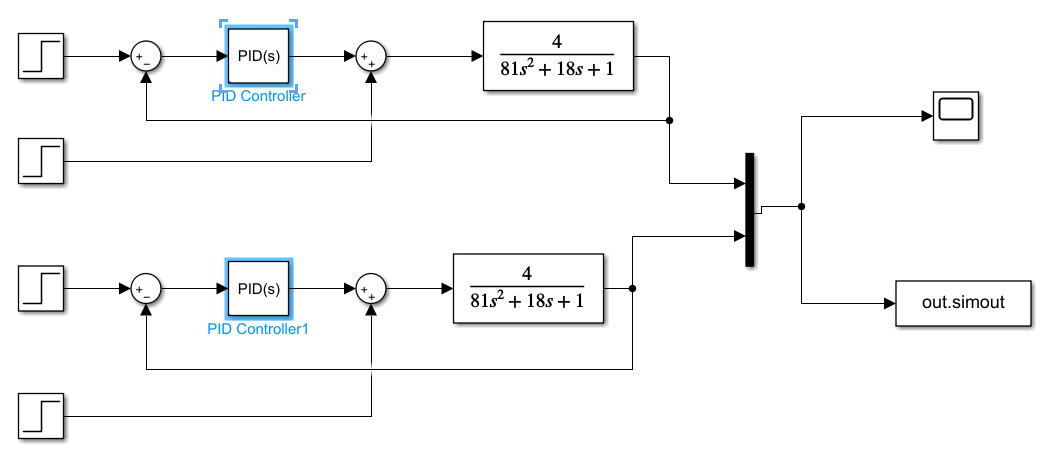
\includegraphics[width=0.5\textwidth]{p4.png}
    \caption{\label{Fig:p4}Simulink Model with 5 disturbance at 70s}
    \end{centering}
    
\end{figure}


Figure \ref{Fig:p4} shows the simulate model of P and PI model with additional disturbance. In this case, for the P model, $K_{p}$ was set to be 9.65 while the $K_{p}$ and $K_{I}$ of PI model was set to be 8.69 and 1.03. After the controller, a disturbance was implemented with a unit-step with amplitude of 5 at 70s. The result was export to the scope for display.

\subsection{Result and Comment}


\begin{figure}[htbp]     \begin{centering}
    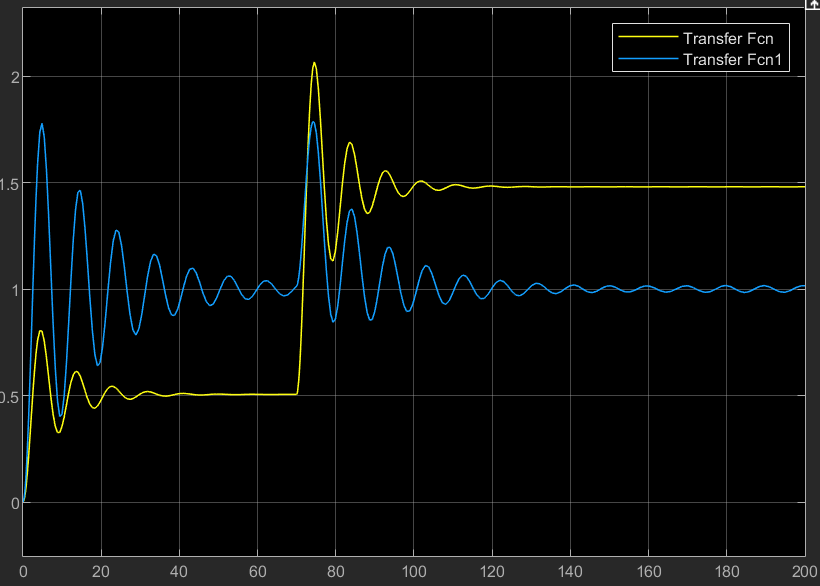
\includegraphics[width=0.5\textwidth]{p4_r.png}
    \caption{\label{Fig:p4_r}Simulink Result with 5 disturbance at 70s}
    \end{centering}
    
\end{figure}


\begin{table}[htbp]
\caption{Disturbance Response of P and PI Model}
\label{tab:resp_4}
\begin{center}
\begin{tabular}{c||ccc}
\hline
Model   &    Max    & $T_{s}$   &  steady error \\
\hline
P  &   2.0   &  102     &  0.47     \\
PI  &   1.7      &  199     &  0     \\
\hline
\end{tabular}
\end{center}
\end{table}

Figure \ref{Fig:p4_r} and Table \ref{tab:resp_4} shows the result of this part. As it can be inferred from Figure \ref{Fig:p4_r}, at 70s, a disturbance was implemented and the system need to recover itself through the P and PI controller. It can be found that comparing with P Model, the PI Model has less Max value, nearly zero steady error while the P Model has a shorter recover time. However, the PI Model is thought to be more suitable for remove the effect of disturbance because its overall performance is better.


\section{Bonus}

\subsection{Method and procedure}

According to the FOPDT case, for a PID controller, the parameters $K_{p}$, $K_{I}$ and $K_{D}$ can be designed as $1.2\frac{T_{p}}{t_{d}}$, $0.6\frac{T_{p}}{t_{d}^2}$ and $0.6T_{p}$ accordingly. In our case, they are 11.52, 2.28 and 14.68.

\begin{figure}[htbp]     \begin{centering}
    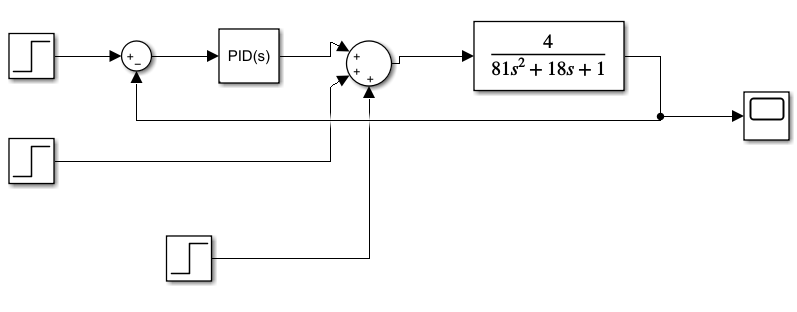
\includegraphics[width=0.5\textwidth]{5.png}
    \caption{\label{Fig:p5}Simulink with 2 disturbance at 70s and 140s}
    \end{centering}
    
\end{figure}

To test the system's ability to against disturbance, 2 unit-step disturbance with amplitude 1 and 5 were implemented at 70s and 140s. The simulink model can be shown in Figure \ref{Fig:p5}.
\newpage

\subsection{Result and Comment}

\begin{figure}[htbp]     \begin{centering}
    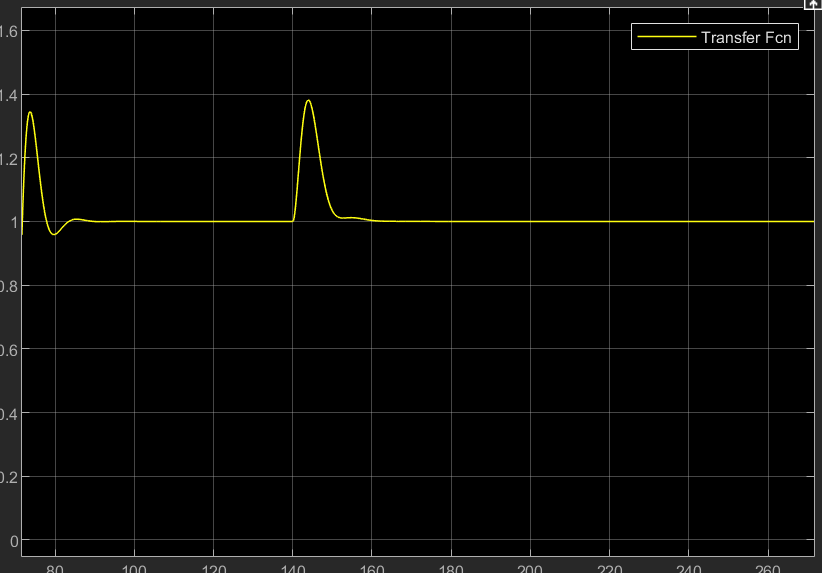
\includegraphics[width=0.5\textwidth]{5_r.png}
    \caption{\label{Fig:p5_r}Simulink Result with 2 disturbance at 70s and 140s}
    \end{centering}
   
\end{figure}

From Figure \ref{Fig:p5_r}, it can be seen that these two disturbance were eliminated successfully. With around 40\% OS\% and $T_{s}$ within 10s, this response was expected.

\section{Discussion and Conclusion}

In this experiment, controller design method has been designed utilizing P model, PI model and PID model. FOPDT method was used to approximate the original response and to find the suitable parameters. It was investigated that comparing with P model, PI model seems to have higher OS\% but with nearly removed steady error. PI model shows more expected ability to against disturbance because of less Max value, nearly zero steady error compared with P model. Finally, a PID model was designed to make the anti-disturbance ability of the system to be as high as possible.

It was discovered that the P component can slightly decrease the system stability and generate fast transient response while resulting in higher steady-state error and overshoot. The I component can improve the stability, decrease the steady-state error and overshoot while giving rise to a longer transient response. The D component can control the overshoot to be smaller but will result in low stability, slow transient response and more steady-state error.



%-------------------------------------------------------------------------------------------------------

\bibliographystyle{IEEEtran}
\bibliography{MyRefs}         % The file MyRefs.bib contains the actual bibliography material
                                  % References section created automatically
\addcontentsline{toc}{section}{References}



% --------------------------- This is how to declare the Appendices section ----------------------------
\newpage
\appendix
\appendixpage
\addappheadtotoc

\section{Part 1 Screenshot}

\begin{figure}[htbp]     \begin{centering}
    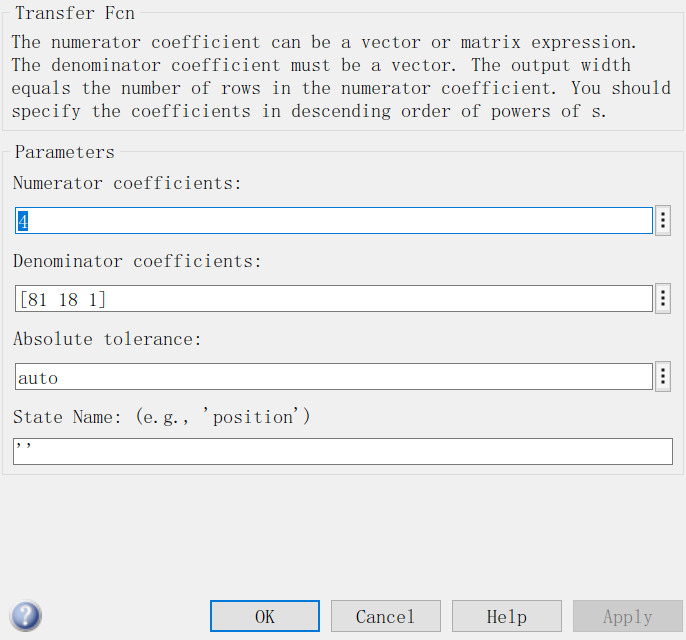
\includegraphics[width=0.5\textwidth]{a1_1.png}
    \caption{Part 1 trans func}
    \end{centering}
\end{figure}

\begin{figure}[htbp]     \begin{centering}
    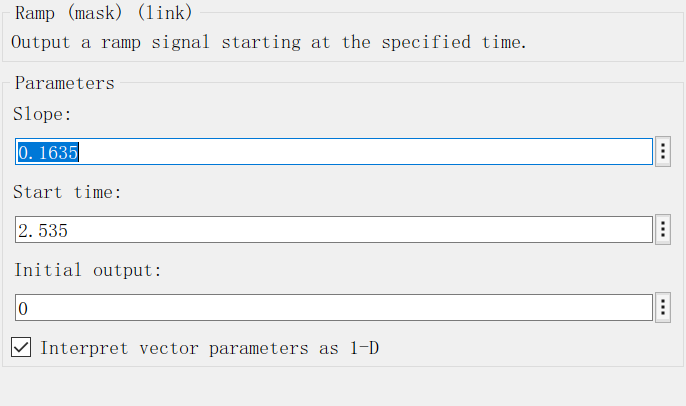
\includegraphics[width=0.5\textwidth]{a1_2.png}
    \caption{Part 1 tangent line}
    \end{centering}
\end{figure}

\begin{figure}[htbp]     \begin{centering}
    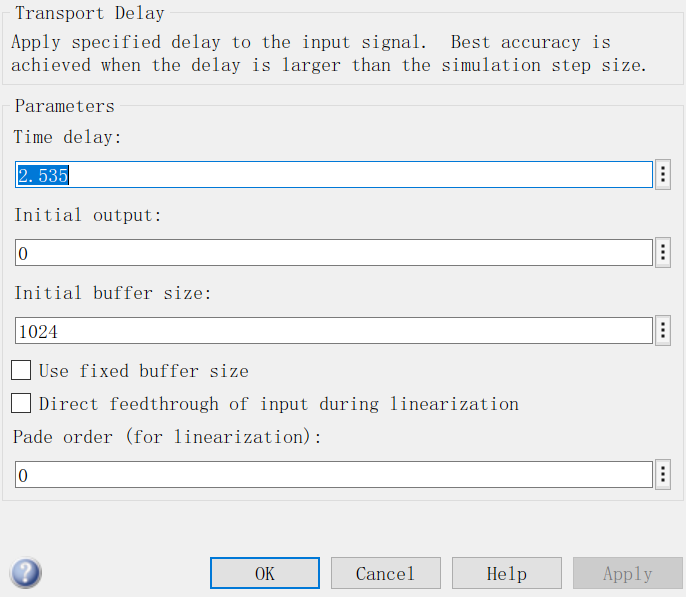
\includegraphics[width=0.5\textwidth]{a1_3.png}
    \caption{Part 1 FOPDT delay module}
    \end{centering}
\end{figure}

\newpage

\section{Part 2 Screenshot}

\begin{figure}[htbp]     \begin{centering}
    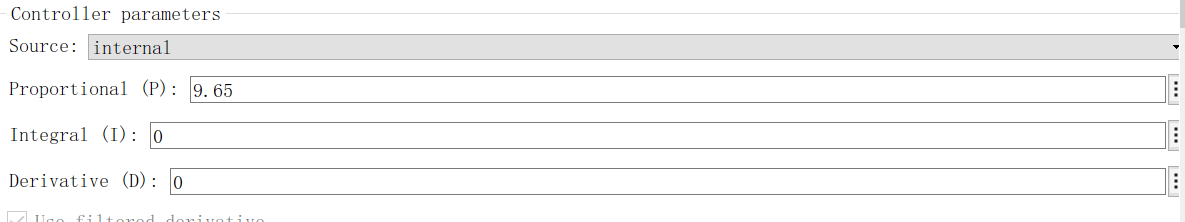
\includegraphics[width=0.5\textwidth]{a2.png}
    \caption{Part 2 P model}
    \end{centering}
\end{figure}

\section{Part 3 Screenshot}

\begin{figure}[htbp]     \begin{centering}
    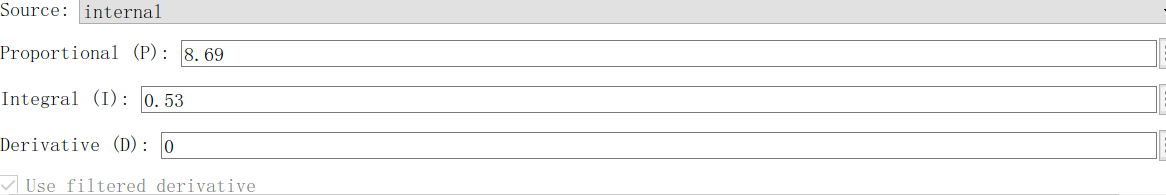
\includegraphics[width=0.5\textwidth]{a3_1_1.png}
    \caption{Part 3 PI Model}
    \end{centering}
\end{figure}

\begin{figure}[htbp]     \begin{centering}
    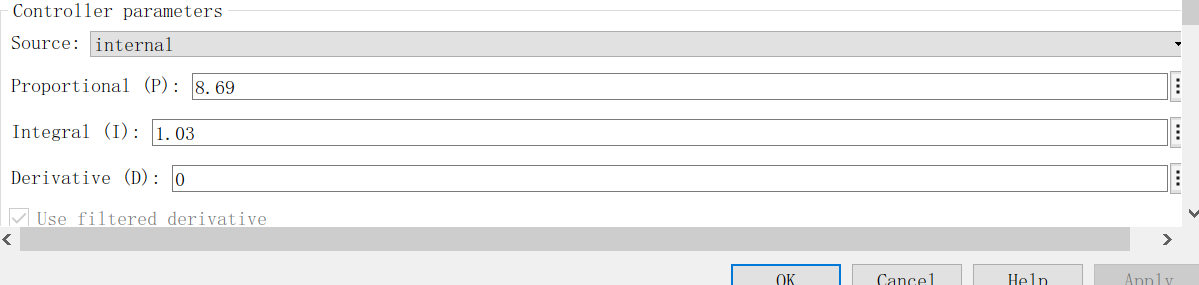
\includegraphics[width=0.5\textwidth]{a3_1_2.png}
    \caption{Part 3 PI Model}
    \end{centering}
\end{figure}

\begin{figure}[htbp]     \begin{centering}
    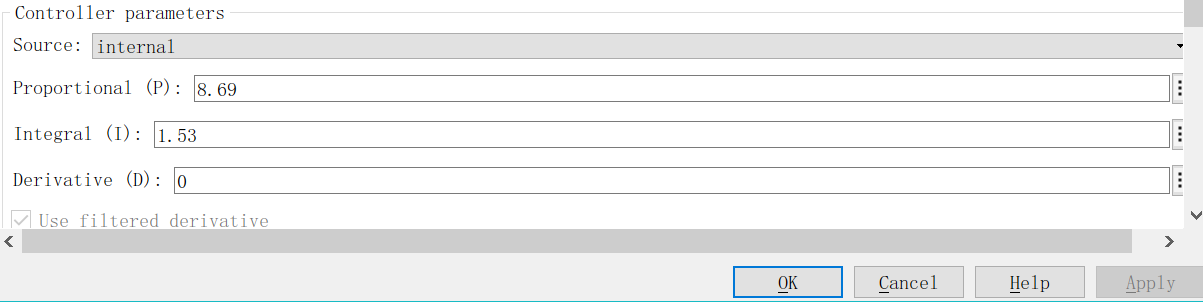
\includegraphics[width=0.5\textwidth]{a3_1_3.png}
    \caption{Part 3 PI Model}
    \end{centering}
\end{figure}

\begin{figure}[htbp]     \begin{centering}
    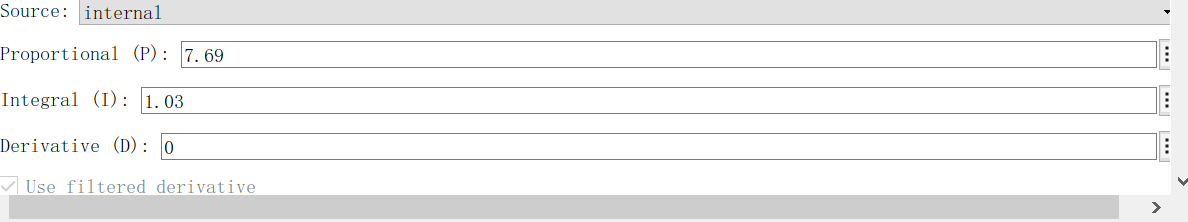
\includegraphics[width=0.5\textwidth]{a3_2_1.png}
    \caption{Part 3 PI Model}
    \end{centering}
\end{figure}

\begin{figure}[htbp]     \begin{centering}
    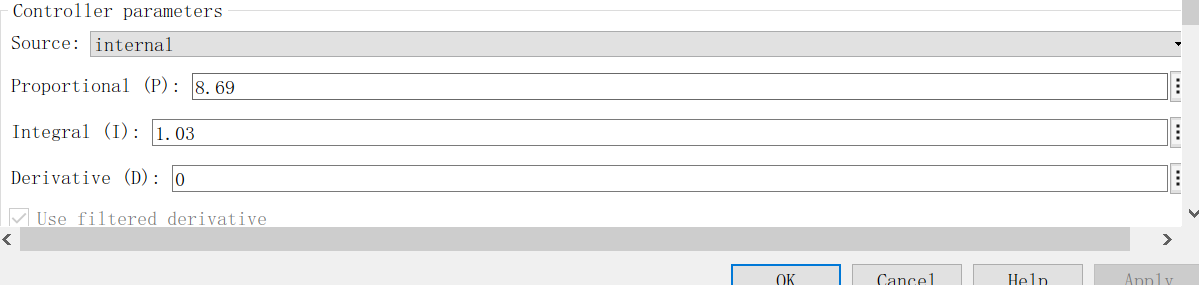
\includegraphics[width=0.5\textwidth]{a3_2_2.png}
    \caption{Part 3 PI Model}
    \end{centering}
\end{figure}

\begin{figure}[htbp]     \begin{centering}
    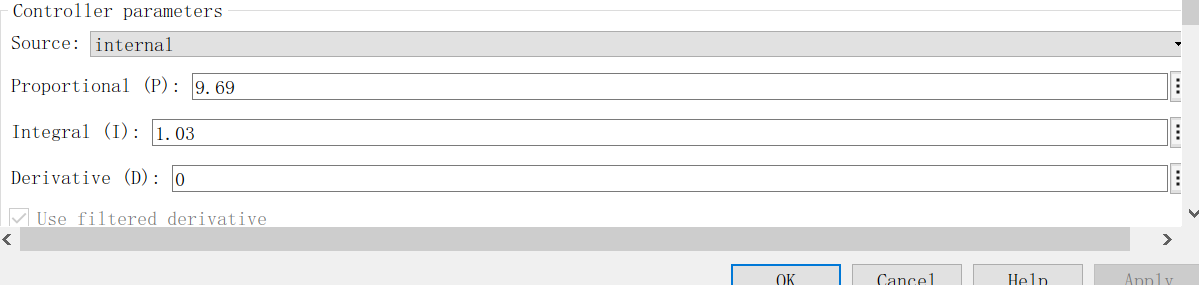
\includegraphics[width=0.5\textwidth]{a3_2_3.png}
    \caption{Part 3 PI Model}
    \end{centering}
\end{figure}

\newpage

\section{Part 4 Screenshot}

\begin{figure}[htbp]     \begin{centering}
    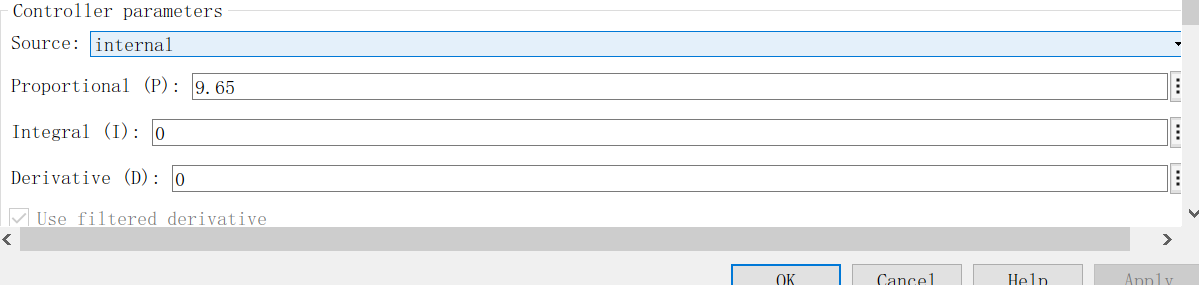
\includegraphics[width=0.5\textwidth]{a4_1.png}
    \caption{Part 4 PI Model}
    \end{centering}
\end{figure}

\begin{figure}[htbp]     \begin{centering}
    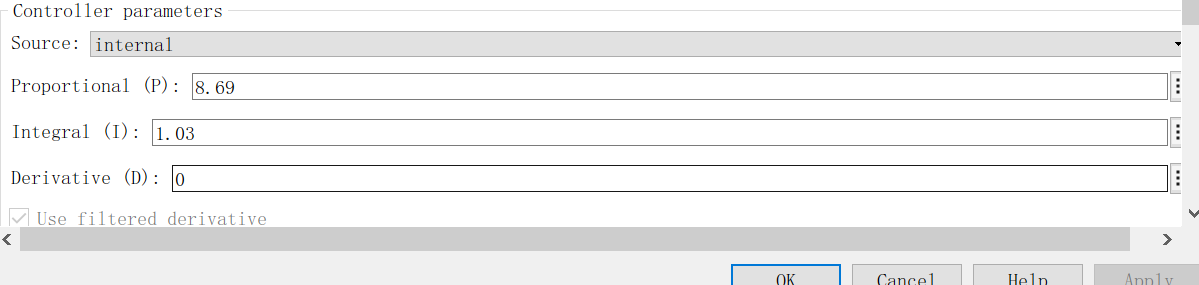
\includegraphics[width=0.5\textwidth]{a4_2.png}
    \caption{Part 4 PI Model}
    \end{centering}
\end{figure}

\begin{figure}[htbp]     \begin{centering}
    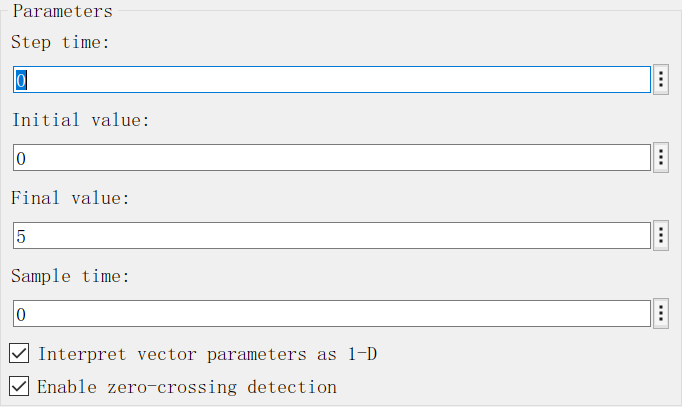
\includegraphics[width=0.5\textwidth]{a4_3.png}
    \caption{Part 4 disturbance}
    \end{centering}
\end{figure}

\begin{figure}[htbp]     \begin{centering}
    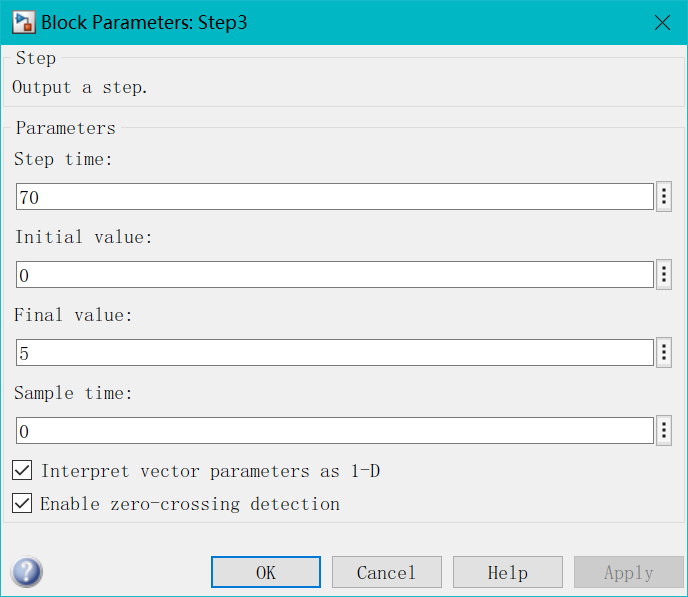
\includegraphics[width=0.5\textwidth]{a4_4.png}
    \caption{Part 4 disturbance}
    \end{centering}
\end{figure}

\newpage
\section{Part 5 Screenshot}

\begin{figure}[htbp]     \begin{centering}
    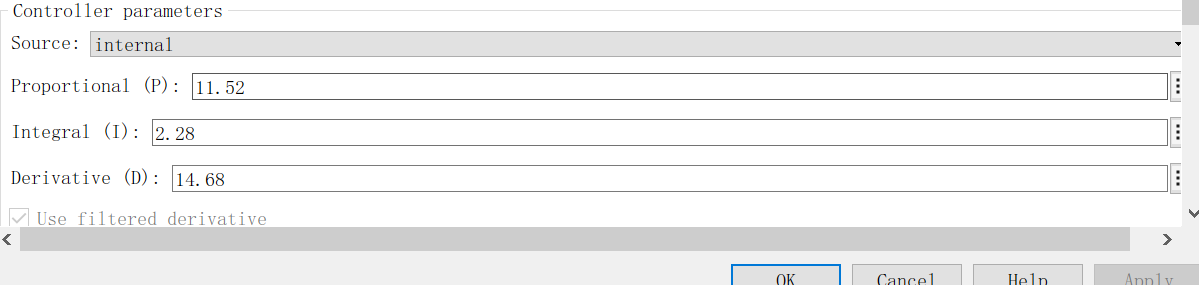
\includegraphics[width=0.5\textwidth]{a5_1.png}
    \caption{Part 5 PID Model}
    \end{centering}
\end{figure}

\begin{figure}[htbp]     \begin{centering}
    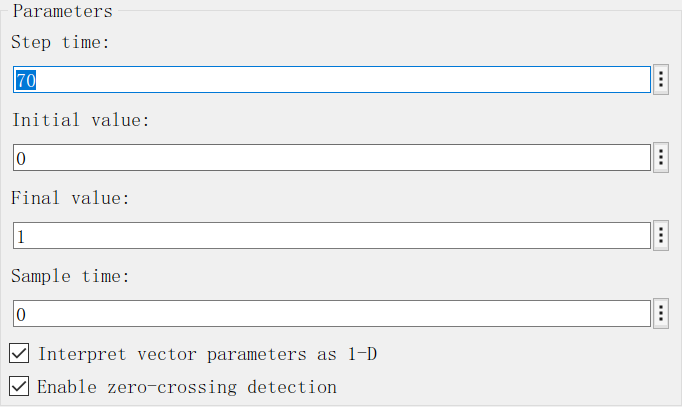
\includegraphics[width=0.5\textwidth]{a5_2.png}
    \caption{Part 5 disturbance}
    \end{centering}
\end{figure}

\begin{figure}[htbp]     \begin{centering}
    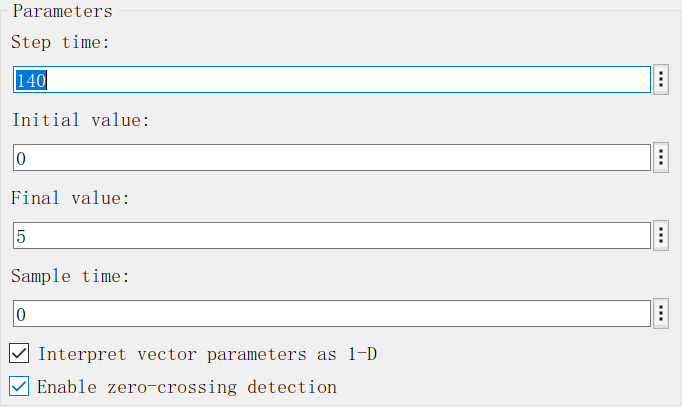
\includegraphics[width=0.5\textwidth]{a5_3.png}
    \caption{Part 5 disturbance}
    \end{centering}
\end{figure}


\end{document}
